\documentclass[11pt,a4paper]{article}
\usepackage[margin=1in]{geometry}
\usepackage[T1]{fontenc}
\usepackage{lmodern,microtype}
\usepackage{amsmath,amssymb,amsthm,booktabs,graphicx}
\usepackage{natbib}
\usepackage{caption,placeins}
\usepackage[colorlinks=true,allcolors=blue!45!black]{hyperref}
\usepackage{xcolor}
\usepackage{setspace}
\setstretch{1.12}
\setlength{\parskip}{3pt}
\setlength{\emergencystretch}{1em}
\renewcommand{\topfraction}{0.9}
\renewcommand{\bottomfraction}{0.9}
\renewcommand{\textfraction}{0.08}
\renewcommand{\floatpagefraction}{0.8}
\setcounter{topnumber}{5}
\setcounter{bottomnumber}{5}
\setcounter{totalnumber}{8}
\setlength{\textfloatsep}{14pt}
\setlength{\intextsep}{12pt}
\setlength{\parindent}{1.2em}
\captionsetup{font=small,labelfont=bf}
\newtheorem{proposition}{Proposition}
\newtheorem{lemma}{Lemma}
\graphicspath{{../figures/}}
\newcommand{\RawRows}{55,754}
\newcommand{\PanelRows}{53,161}
\newcommand{\QuarantineRows}{2,593}
\newcommand{\SwissBefore}{44.26}
\newcommand{\SwissAfter}{61.21}
\newcommand{\SwissChange}{16.94}
\newcommand{\LowerBound}{54.91}
\newcommand{\UpperBound}{65.34}
\newcommand{\MinSelection}{10.65}
\newcommand{\AgriChange}{-0.81}
\newcommand{\AgriRate}{-0.86}
\newcommand{\PanelCount}{184}
\newcommand{\ReversalCount}{16}
\newcommand{\EligibleFall}{92.52}
\newcommand{\UnusedBefore}{1,060.71}
\newcommand{\UnusedAfter}{55.22}

\title{Tariff Abolition and the Measurement\\of Trade-Agreement Use}
\author{Shivam Gupta\\\normalsize Independent Researcher\\\normalsize\texttt{shivam1720406@gmail.com}}
\date{16 October 2026}
\begin{document}
\maketitle
\begin{abstract}
Does an increase in preference utilization indicate better use of a trade agreement when tariff liberalization removes goods from preference eligibility? We examine this question using the United Kingdom's published tariff-regime databases and Switzerland's 2024 abolition of industrial import tariffs. UK exports to Switzerland recorded a utilization increase from \SwissBefore\% to \SwissAfter\%, while eligible trade fell by \EligibleFall\%. In agricultural chapters 01--24, utilization instead declined by 0.81 percentage point. An exact common-support decomposition assigns the aggregate increase to eligibility exit and changing chapter weights, with a negative within-chapter rate component. A frozen-2023-basket exercise treats the agricultural exceptions in chapters 35 and 38 as unresolved rather than misclassifying them. Sharp accounting bounds put post-removal utilization between \LowerBound\% and \UpperBound\%, containing the observed 2024 rate without requiring a change in claiming behavior. In a broader matched panel, \ReversalCount\ of \PanelCount\ material partner--direction--year comparisons have opposing aggregate and within-chapter rate changes. We provide proofs, exact-arithmetic and optimization checks, a source-year quarantine, and an open replication package. The contribution is a reproducible assessment of selection in agreement-use statistics, with implications for policy evaluation and trade-compliance performance reporting.
\end{abstract}
\noindent\textbf{Keywords:} preference utilization; tariff liberalization; rules of origin; trade-agreement evaluation; composition effects.\\
\textbf{JEL codes:} F13, F14, F15, C43.\\
\textbf{Research materials:} \url{https://github.com/shi1720/preference-selection}.

\section{Introduction}
A trade agreement can become less necessary for obtaining duty-free access even while its reported utilization improves. The reason is institutional. Preference utilization is conditional on an available tariff advantage. When the most-favoured-nation (MFN) tariff falls to zero, claiming a preferential tariff no longer generates that advantage, and the corresponding goods leave the utilization denominator. An evaluation that interprets an increase in the remaining ratio as improved implementation can consequently reward a change in the population being measured.

This issue has a concrete policy setting. Switzerland abolished industrial import tariffs on 1 January 2024. Most products in Harmonized System (HS) chapters 25--97 became duty-free regardless of origin. Agriculture remained protected, including specific agricultural products in chapters 35 and 38 \citep{seco2026}. For UK exports to Switzerland, the published databases imply that preference utilization rose from \SwissBefore\% in 2023 to \SwissAfter\% in 2024. Yet utilization in chapters 01--24 declined from 62.04\% to 61.23\%. The headline increase and the agricultural decline are both correct descriptions of different changing trade aggregates.

We ask three questions. How much of the observed change comes from rates within continuing eligible chapters, from changing weights, and from aggregate eligibility entry or exit? Can the sign and scale of the Swiss increase be reproduced by eligibility selection alone on a fixed historical basket? How often do aggregate and within-chapter rate changes point in opposite directions elsewhere in the public UK data?

We answer the first question through an exact decomposition that separates common-support rates and weights from eligibility entry and exit. The rate--weight split is the classical symmetric decomposition of \citet{kitagawa1955}; the contribution lies in its application with an explicit eligibility-support ledger, rather than a new decomposition theorem. For Switzerland in 2023--24, the aggregate increase of 16.94 percentage points comprises a rate contribution of $-4.68$ points, a weight contribution of $+7.46$ points, and an aggregate eligibility-exit contribution of $+14.16$ points. The rate component remains an aggregate chapter statistic. It cannot identify changes in an individual firm's probability of claiming a preference.

For the second question, we construct a frozen-basket benchmark. We remove the chapters certainly covered by the industrial reform, retain chapters 01--24, and leave the allocation of eligible trade within mixed chapters 35 and 38 unresolved. We derive sharp upper and lower bounds under exactly that coarse information set. On the 2023 basket, the resulting interval is [\LowerBound\%, \UpperBound\%]. Its lower endpoint already exceeds the pre-reform rate by \MinSelection\ points. The observed 2024 rate lies inside it. This is a constructive demonstration that the headline increase is compatible with no improvement in claiming on the frozen basket. It is not an estimate, or a bound, for the realized causal contribution of the reform.

For the third question, we analyze matched partner--direction panels in 2022--23 and 2023--24. Requiring at least \pounds100 million in eligible trade in both years and at least 99\% eligibility coverage on matched chapters leaves \PanelCount\ comparisons. In \ReversalCount\, aggregate and within-chapter rate changes have opposite signs and both exceed 0.5 percentage point in magnitude. These are descriptive comparisons, with repeated partners and non-random country coverage. The results establish that the Swiss concern is not confined to a numerical curiosity, while also showing why its precise diagnosis requires policy information.

The analysis has a bounded contribution. Official statistics already distinguish preference use from tariff-free trade and acknowledge the Swiss eligibility change. Existing research already establishes that compliance costs, origin requirements, margins, experience, and trade composition matter. Our contribution is the quantified Swiss reversal, a transparent treatment of mixed-chapter uncertainty, and a reproducible comparison of aggregate and common-support changes across public tables. We do not identify new firm-level learning effects, estimate welfare, or claim a general solution to trade-agreement evaluation.

\section{Related research and institutional setting}
\subsection{Preference use, costs, and composition}
The literature provides strong reasons to avoid treating non-use as a simple information deficit. \citet{keck2012} documents the importance of fixed utilization costs. \citet{legge2024} studies transaction-level Swiss imports and finds a fixed-cost component, particularly for urgent shipments. \citet{krishna2025} identifies learning in preference use with exporter--importer transaction data. These studies investigate behavior with information unavailable in the published chapter tables analyzed here.

Origin requirements can also affect the organization of production. \citet{conconi2018} demonstrates that rules of origin can redirect intermediate-input sourcing. \citet{cariola2022} relates preference utilization to value-added content and effective preference margins. These findings distinguish legal access to a preferential schedule from the ability and incentive to meet its origin conditions. Published eligibility therefore does not establish that every non-claiming shipment could profitably qualify.

For post-Brexit trade, \citet{ayele2023} constructs a rules-of-origin restrictiveness index and studies product-level utilization. \citet{tamberi2022} discusses TCA utilization and the role of composition; \citet{brenis2024} compares the use of several UK agreements. \citet{ons2025} provides firm-level evidence for UK imports. Our analysis does not replace these explanations. It examines an earlier measurement step: whether a change in the aggregate conditional ratio has the same sign as the rate change within continuing eligible groups.

Neither tariff-free trade nor decomposing trade into tariff regimes is new. \citet{gonciarz2025} provides a comprehensive analysis of MFN and preferential trade, and DBT publishes both preference utilization and tariff-free shares. Likewise, SECO's agreement-use monitoring includes realized tariff savings \citep{secomonitor2026}. Our proposed reporting treatment uses established measures together, with explicit support changes and uncertainty, rather than introducing a new headline index.

\subsection{Why the Swiss reform is informative}
The Swiss measure changed the basis on which many imports obtained duty-free access. It was unilateral, applying across origins, while foreign tariffs on Swiss exports remained. The reform left customs-declaration obligations and other taxes in place. Proof of preferential origin ceased to be necessary for industrial imports expected to remain in Switzerland, although origin documentation can still matter for re-export or cumulation \citep{seco2026}. Thus the reform can reduce the need for a preference claim without removing all trade administration.

This is a particularly clear setting for a measurement exercise because it changes eligibility on a known date and across a large product range. It is less suitable for an aggregate before--after estimate of compliance learning. Product composition, prices, firms, processing arrangements, and sourcing can change at the same time. We use the legal change to classify certain and ambiguous removal, not to assume these other margins away in the realized data.

DBT's 2024 commentary explicitly notes the sharp reduction in UK exports eligible for preferences in Switzerland \citep{dbt2026b}. The empirical claim here is therefore more specific than discovering that eligibility fell: the aggregate rate increase coexists with a decline in the agricultural rate; its four accounting components can be reconstructed; and even the agricultural exceptions cannot overturn the positive frozen-basket selection effect under the specified information set.

\section{Data, provenance, and comparison universe}
\subsection{Official databases and units}
We archive the eight import and export databases in DBT's 2021--2024 preference-utilization collection, retrieved on 16 October 2026 \citep{dbt2026a}. These are ODS workbooks with partner--HS2 records. The package preserves their bytes, release-page and download URLs, SHA-256 hashes, and parsed numeric fields. It contains \RawRows\ source records. Values are current pounds sterling; export records supplied in foreign currencies are converted in the official publication. We calculate ratios from the value fields, not from the separately rounded percentage columns.

For cell $i$ in year $t$, let $E_{it}$ be preference-eligible value and $P_{it}$ value using preferences. We define unused eligible value as $E_{it}-P_{it}$. Eligibility in these tables concerns an available tariff advantage under the statistical methodology. It does not certify satisfaction of all origin requirements for each shipment. Special-processing and unknown-regime trade are excluded from the relevant utilization universe \citep{dbtannex2026}.

The separate duty-free share combines MFN-zero, FTA-zero and, for imports, development-scheme-zero entries over known normal-regime trade. A positive preferential tariff counts as preference use but does not count as duty-free entry. We retain this distinction throughout. Neither eligible value nor unused eligible value is a monetary estimate of duties paid or foregone savings.

\begin{table}[!htbp]
\centering
\caption{Source coverage and the year-consistency screen}\label{tab:coverage}
\small
\begin{tabular}{llrrrr}
\toprule
Year & Direction & Source rows & Quarantined & Retained & Partners \\
\midrule
2021 & exports & 4,395 & 2,593 & 1,802 & 21 \\
2021 & imports & 9,070 & 0 & 9,070 & 228 \\
2022 & exports & 4,379 & 0 & 4,379 & 48 \\
2022 & imports & 10,137 & 0 & 10,137 & 235 \\
2023 & exports & 4,171 & 0 & 4,171 & 46 \\
2023 & imports & 9,897 & 0 & 9,897 & 235 \\
2024 & exports & 4,033 & 0 & 4,033 & 44 \\
2024 & imports & 9,672 & 0 & 9,672 & 231 \\
\bottomrule
\end{tabular}
\par\vspace{3pt}\begin{minipage}{.97\linewidth}\footnotesize Partner counts refer to retained records and include partners with no positive eligibility. The 2021 export workbook has 2,593 records whose Year field says 2023. These records are archived but excluded. All other records pass the file-year check. Source: DBT databases retrieved on 16 October 2026 and calculations.\end{minipage}
\end{table}


\subsection{A source-year inconsistency and its treatment}
The current 2021 export workbook contains \QuarantineRows\ rows whose Year field says 2023. The remaining 1,802 rows identify 2021. We do not overwrite the inconsistent field or infer the correct year from the surrounding workbook. Those \QuarantineRows\ rows are retained in a quarantine file and excluded from analysis. This leaves \PanelRows\ records whose file year and declared year agree. The mismatch is a provenance finding, not evidence that the underlying trade values are incorrect. It also cannot be repaired by treating the rows as additional 2023 observations.

All Switzerland records used in the four-year case study pass this screen. The broader comparison uses only 2022--23 and 2023--24. Table~\ref{tab:coverage} reports source and retained coverage separately. The retained data have no duplicate partner--chapter--year--direction keys, negative monetary values, missing eligible/use values, or records with use exceeding eligibility. Other fields are handled with their own completeness requirements rather than turning blanks into zero.

The import series has an additional comparability issue. Staged customs controls affected 2021 EU-to-Great-Britain reporting; the official technical annex cautions against straightforward cross-year interpretation \citep{dbtannex2026}. This supports using 2022 onward for the broader analysis. Country coverage for exports also changes as partners provide data. We compare each partner only on explicitly observed matched chapter rows.

\subsection{Matching, materiality, and inference}
For any two years, we take an inner join on partner and chapter within a trade direction. A missing row does not become a zero-eligibility record. This is necessary because data-exchange coverage, reporting, and zero trade are different events. Eligibility entry and exit below refer only to observed matched cells changing between a positive and an explicitly recorded zero denominator.

For the broader descriptive panel, both years must have at least \pounds100 million in matched eligible value. Matched chapters must cover at least 99\% of all reported eligibility in each year. These thresholds are transparent choices for avoiding tiny denominators and material coverage changes; they were not preregistered. We report alternative value thresholds and change thresholds. The full output includes panels that do not exhibit a reversal.

These data are administrative aggregates, not an independent sample of firms or agreements. We do not attach sampling standard errors to accounting identities or interpret repeated partner comparisons as independent experimental units. Numerical checks assess implementation. Sensitivity exercises assess the dependence of the descriptive conclusions on the comparison universe and weighting convention.

\section{Accounting framework}
\subsection{Why deleting eligibility can raise utilization}
For a positive eligible total $E$ and used total $P$, write $U=P/E$. Suppose a tariff reform removes eligible value $d$ with used-preference value $q$, holding the remaining basket fixed. If $0<d<E$, the new utilization ratio is $(P-q)/(E-d)$ and
\begin{equation}
 \frac{P-q}{E-d}-\frac PE
 =\frac{d}{E-d}\left(U-\frac qd\right).
 \label{eq:deletion}
\end{equation}
Utilization rises precisely when the removed pool had below-average utilization. The identity says nothing about whether the reform improves claiming behavior among retained transactions. It is a general property of a selected ratio, not a new behavioral result.

\subsection{Common support with eligibility entry and exit}
Within the matched row universe, let $K$ contain cells with positive eligibility in both years, $D$ cells eligible only in year 0, and $N$ cells eligible only in year 1. Let $E_t$ be total eligibility, $E_{Kt}$ the common-support total, and $u_{Kt}=P_{Kt}/E_{Kt}$. Assume $E_{Kt}>0$. For $i\in K$, define $u_{it}=P_{it}/E_{it}$ and $w_{it}=E_{it}/E_{Kt}$.

\begin{lemma}[Exact support decomposition]
The aggregate utilization change satisfies
\begin{align}
 U_1-U_0 &= R+W+X+A,\label{eq:split}\\
 R&=\sum_{i\in K}\frac{w_{i0}+w_{i1}}2(u_{i1}-u_{i0}),\label{eq:rate}\\
 W&=\sum_{i\in K}\frac{u_{i0}+u_{i1}}2(w_{i1}-w_{i0}),\\
 X&=\frac{E_{D0}u_{K0}-P_{D0}}{E_0},\qquad
 A=\frac{P_{N1}-E_{N1}u_{K1}}{E_1}.\label{eq:support}
\end{align}
Empty entry and exit pools contribute zero.
\end{lemma}
\begin{proof}
Write $U_0=u_{K0}+(P_{D0}-E_{D0}u_{K0})/E_0$ and $U_1=u_{K1}+(P_{N1}-E_{N1}u_{K1})/E_1$. Subtraction gives $U_1-U_0=(u_{K1}-u_{K0})+X+A$. Expanding $u_{K1}-u_{K0}=\sum_K(w_{i1}u_{i1}-w_{i0}u_{i0})$ with the symmetric product identity yields $R+W$.
\end{proof}

The symmetric split in equations~\eqref{eq:rate}--\eqref{eq:support} uses the familiar rate-standardization logic of \citet{kitagawa1955}. $X$ is positive when exiting chapters used preferences less than the common-support baseline average. $A$ is positive when entering chapters use preferences more than the common-support final average. Changing the normalization or the order of sequential replacements can allocate interaction terms differently. We state this convention so that the reported components are reproducible.

Three interpretation limits matter. First, cell-level exit can reflect demand and composition as well as legal policy, unless the policy supplies an independent reason for the exit. Second, common support is defined at HS2. A positive chapter denominator can conceal tariff-line entry and exit within it. Third, the chapter's rate component includes changes in the mix of firms, products, shipment values, and origin eligibility. Calling $R$ ``learning'' or ``implementation effectiveness'' would exceed what the data identify.

\subsection{Sharp bounds with mixed product chapters}
The Swiss reform leaves uncertainty if only HS2 data are available. Partition the baseline basket into a certainly retained pool, a certainly removed pool, and an ambiguous pool. Let retained eligibility and use be $(e,p)$, with $e>0$, and ambiguous eligibility and use be $(a,q)$, with $0\leq q\leq a$. In the ambiguous pool, let $v$ be used value retained after applying the policy classification and $w$ unused eligible value retained. The available information imposes
\begin{equation}
 0\leq v\leq q,\qquad 0\leq w\leq a-q.
 \label{eq:ambiguous}
\end{equation}
The post-removal frozen-basket ratio is
\begin{equation}
 U^{\mathrm{sel}}(v,w)=\frac{p+v}{e+v+w}.
 \label{eq:selection}
\end{equation}
All pre-policy values and claim assignments are held fixed. The exercise changes only whether those values remain in the denominator.

\begin{proposition}[Mixed-pool selection interval]
Under~\eqref{eq:ambiguous}, the attainable ratios form the closed interval
\begin{equation}
 \left[\frac{p}{e+a-q},\quad\frac{p+q}{e+q}\right].
 \label{eq:bounds}
\end{equation}
If total ambiguous retention is known to be $r\in[0,a]$, the interval becomes
\begin{equation}
 \left[\frac{p+\max\{0,r-(a-q)\}}{e+r},\quad
       \frac{p+\min\{r,q\}}{e+r}\right].
 \label{eq:fixed}
\end{equation}
These bounds are sharp relative to the stated aggregate information.
\end{proposition}
\begin{proof}
The ratio is weakly increasing in $v$ and weakly decreasing in $w$, since $0\leq p\leq e$. Its extrema are attained at $(v,w)=(0,a-q)$ and $(q,0)$. The feasible rectangle is connected and the ratio continuous, so every intermediate value is attained. Conditional on $v+w=r$, feasibility requires $\max\{0,r-(a-q)\}\leq v\leq\min\{r,q\}$; the denominator is fixed and the numerator increases in $v$.
\end{proof}

This is an accounting relaxation of unresolved tariff-line composition. It does not assert that any arbitrary retention pattern is legally feasible under the full Swiss tariff schedule. Additional tariff-line classifications can narrow the feasible rectangle and hence tighten the interval. In particular, the small observed 2024 residual in mixed chapters is not the value of their retained 2023 basket. Equating the two would assume away changes in quantities, prices, and product composition.

\section{Results for UK exports to Switzerland}
\subsection{The aggregate improvement and the surviving agricultural margin}
Table~\ref{tab:swiss} and Figure~\ref{fig:rates} show the change in the measured population. Eligible value fell from \pounds1,902.98 million in 2023 to \pounds142.34 million in 2024, a \EligibleFall\% decline. Used-preference value fell from \pounds842.27 million to \pounds87.12 million. Both numerator and denominator contracted; the denominator contracted more strongly. The utilization ratio consequently increased by \SwissChange\ percentage points.

\begin{table}[!htbp]
\centering
\caption{UK exports to Switzerland: eligibility, use, and duty-free access}\label{tab:swiss}
\small
\begin{tabular}{lrrrrrr}
\toprule
 & \multicolumn{3}{c}{All chapters} & \multicolumn{2}{c}{Chapters 01--24} & Duty-free \\
Year & Eligible & Used & PUR (\%) & Eligible & PUR (\%) & share (\%) \\
\midrule
2021 & 1,979.71 & 680.97 & 34.40 & 127.85 & 65.71 & 94.78 \\
2022 & 2,289.57 & 853.13 & 37.26 & 137.18 & 70.49 & 68.02 \\
2023 & 1,902.98 & 842.27 & 44.26 & 146.99 & 62.04 & 74.18 \\
2024 & 142.34 & 87.12 & 61.21 & 142.28 & 61.23 & 97.48 \\
\bottomrule
\end{tabular}
\par\vspace{3pt}\begin{minipage}{.97\linewidth}\footnotesize Values are GBP million at each year's prices and conversion rate. Duty-free access uses known normal-regime trade, excludes special processing and unknown regimes, and combines MFN-zero and preferential-zero entries. It is not a measure of non-tariff barriers or a welfare index. The Swiss series passes the year-consistency screen in every year.\end{minipage}
\end{table}

\begin{figure}[!htbp]
\centering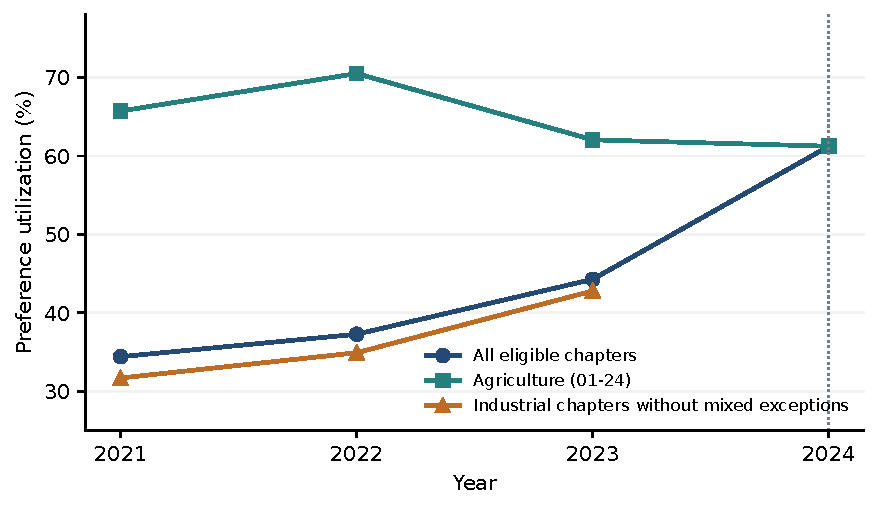
\includegraphics[width=.92\linewidth]{01_swiss_rates.pdf}
\caption{Preference utilization in UK exports to Switzerland. The industrial line excludes mixed chapters 35 and 38 and ends in 2023 because its 2024 eligible denominator is zero. The absence of a 2024 ratio is substantive, not a zero utilization observation. Source: archived DBT databases and calculations.}\label{fig:rates}
\end{figure}

In chapters 01--24, eligibility changed much less, from \pounds146.99 million to \pounds142.28 million, and utilization declined by 0.81 point. The two aggregates therefore provide opposite directional descriptions. The agricultural comparison does not establish that industrial claimants would have behaved similarly in the absence of the reform. It measures the surviving sectoral margin directly.

Figure~\ref{fig:mass} separates used and unused eligible value across the legal product groups. The certain-removal chapters contain \pounds1,722.89 million of 2023 eligibility, including \pounds985.82 million unused. Their 2024 eligibility is zero. Chapters 35 and 38 contain \pounds33.09 million of baseline eligibility, of which \pounds14.00 million used a preference. Their 2024 residual is only \pounds0.051 million, with no recorded preference use. The mixed chapters are quantitatively small relative to the pre-reform industrial basket, but material relative to the post-reform denominator. Treating both chapters as entirely industrial would miss that distinction.

\begin{figure}[!htbp]
\centering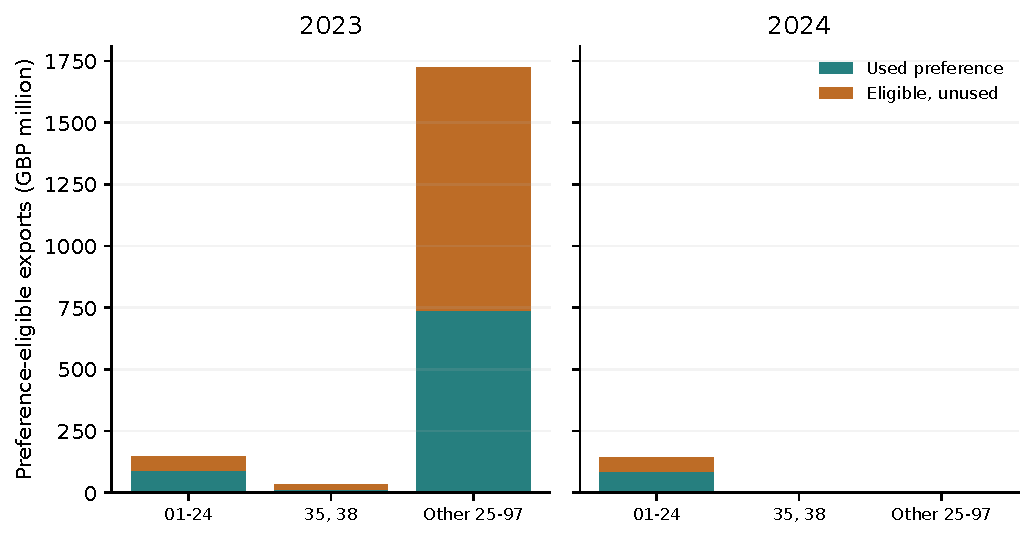
\includegraphics[width=\linewidth]{02_eligible_mass.pdf}
\caption{Eligible export value before and after the Swiss reform. Bars distinguish preference use from eligible non-use, in GBP million. The common vertical scale makes the collapse of industrial eligibility visible. ``Other 25--97'' excludes chapters 35 and 38. Eligible non-use is trade value, not a duty-saving estimate.}\label{fig:mass}
\end{figure}

The unused eligible total fell from \pounds\UnusedBefore\ million to \pounds\UnusedAfter\ million. That difference cannot be described as successful recovery of formerly unclaimed preferences. A large portion of the former pool no longer needed preferential tariff treatment. At the same time, the duty-free share of known normal-regime exports rose from 74.18\% to 97.48\%. Tariff-free access and preference use record different routes to lower duties.

\subsection{The exact accounting components}
The full Swiss comparison matches all 96 reported chapter rows and covers 100\% of reported eligibility in both years. Eighteen chapters have positive eligibility in both years; 71 move from positive eligibility to an explicitly recorded zero. Seven have zero eligibility in both years. Table~\ref{tab:decomposition} reports the full decomposition and the agricultural restriction.

\begin{table}[!htbp]
\centering
\caption{Changes in Swiss-market utilization, in percentage points}\label{tab:decomposition}
\small
\begin{tabular}{lrrrrr}
\toprule
Period & Total & Rates & Weights & Exit & Entry \\
\midrule
2021--22 & +2.86 & +2.62 & +0.27 & -0.00 & -0.02 \\
2022--23 & +7.00 & +0.93 & +6.07 & +0.00 & -0.00 \\
2023--24 & +16.94 & -4.68 & +7.46 & +14.16 & +0.00 \\
2023--24, 01--24 & -0.81 & -0.86 & +0.04 & +0.01 & +0.00 \\
\bottomrule
\end{tabular}
\par\vspace{3pt}\begin{minipage}{.97\linewidth}\footnotesize Rates and weights are normalized on common eligible support. Exit and entry are exact accounting adjustments for aggregate cells changing eligibility status. Rates include within-chapter product and firm composition. The entries are not causal effects. Components use unrounded values; displayed sums can differ by 0.01 percentage point.\end{minipage}
\end{table}

\begin{figure}[!htbp]
\centering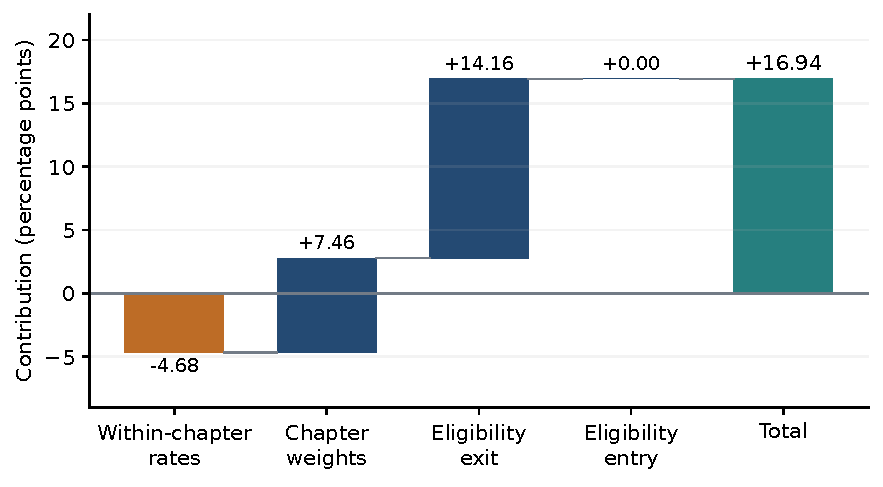
\includegraphics[width=.94\linewidth]{04_decomposition.pdf}
\caption{Accounting for the 2023--24 Swiss-market utilization increase. The negative within-chapter rate component is offset by changing chapter weights and aggregate eligibility exit. The waterfall represents equation~\eqref{eq:split}, not separate causal treatment effects.}\label{fig:decomposition}
\end{figure}

For 2023--24, the exit component contributes 14.16 points, while the continuing-support rate and weight components contribute $-4.68$ and $+7.46$ points. Together they reproduce the 16.94-point headline increase. The common-support aggregate rate itself rises from 58.42\% to 61.21\%, even though its symmetric rate component is negative. This second reversal arises because common-support weights also change substantially. Restricting to continuing chapters is therefore insufficient to remove composition effects.

Within chapters 01--24, 16 have positive eligibility in both years. Four small chapters exit eligibility, contributing only 0.009 point. The rate component is $-0.864$ point, the weight component $+0.043$ point, and the total change $-0.812$ point. This restriction supplies a more stable trade-value comparison, although it still does not track identical tariff lines, firms, or shipments.

The earlier Swiss comparisons offer context. Between 2022 and 2023, aggregate utilization rose by 7.00 points, while the symmetric rate component was only 0.93 point and the weight component 6.07 points. Composition was already relevant before the 2024 abolition. This result is another reason not to label every pre-reform aggregate rise as learning and every post-reform rise as liberalization.

\subsection{What selection alone can reproduce}
For the 2023 frozen basket, set $e=\pounds146.99$ million and $p=\pounds91.19$ million for chapters 01--24, and $a=\pounds33.09$ million and $q=\pounds14.00$ million for chapters 35 and 38. Remove the remaining chapters 25--97. Equation~\eqref{eq:bounds} yields [\LowerBound\%, \UpperBound\%]. Removing only the certainly covered chapters while retaining both mixed chapters gives 58.41\%. Removing both mixed chapters as well gives the agricultural rate, 62.04\%.

\begin{table}[!htbp]
\centering
\caption{Frozen-basket utilization after industrial tariff abolition}\label{tab:bounds}
\small
\begin{tabular}{lrrrr}
\toprule
Base year & Observed PUR & Lower bound & Upper bound & Minimum increase \\
\midrule
2021 & 34.40 & 56.30 & 71.30 & +21.91 \\
2022 & 37.26 & 57.31 & 75.03 & +20.05 \\
2023 & 44.26 & 54.91 & 65.34 & +10.65 \\
\bottomrule
\end{tabular}
\par\vspace{3pt}\begin{minipage}{.97\linewidth}\footnotesize All entries are percentages or percentage-point changes. Retain chapters 01--24, remove chapters 25--97 except 35 and 38, and allow any used/unused split of retained eligibility within the two mixed chapters. These are sharp accounting bounds under that information set. They are not bounds on the realized causal effect of reform. The observed 2024 PUR is 61.21\%.\end{minipage}
\end{table}

\begin{figure}[!htbp]
\centering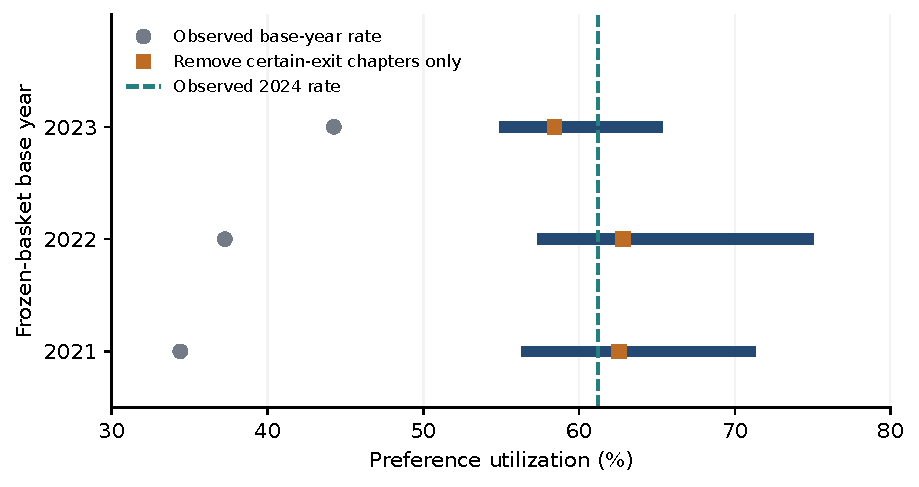
\includegraphics[width=.94\linewidth]{03_retention_bounds.pdf}
\caption{Sharp aggregate-information bounds for frozen-basket selection. Each interval holds that base year's values and preference claims fixed, retains chapters 01--24, removes certain-exit chapters, and permits unresolved allocation within chapters 35 and 38. The dashed line is the realized 2024 rate; overlap is a compatibility result.}\label{fig:bounds}
\end{figure}

The observed \SwissAfter\% rate lies inside the interval. More constructively, it can be matched while retaining no used-preference value from the ambiguous pool and retaining approximately \pounds2.00 million of its unused eligible value. That is feasible because the ambiguous pool contains \pounds19.09 million of unused eligibility. This witness is consistent with the coarse accounting constraints; it is not a reconstruction of the actual legal tariff lines retained.

The baseline-year sensitivity in Table~\ref{tab:bounds} reaches the same compatibility conclusion for 2021 and 2022. These comparisons apply the 2024 removal classification to historical baskets. They do not estimate pre-trends or the behavior of treated firms. Figure~\ref{fig:fixed} shows the more informative conditional bounds if external tariff-line work supplies the amount $r$ of mixed-chapter baseline eligibility retained. The interval contracts to a point when none or all of that pool is retained.

\begin{figure}[!htbp]
\centering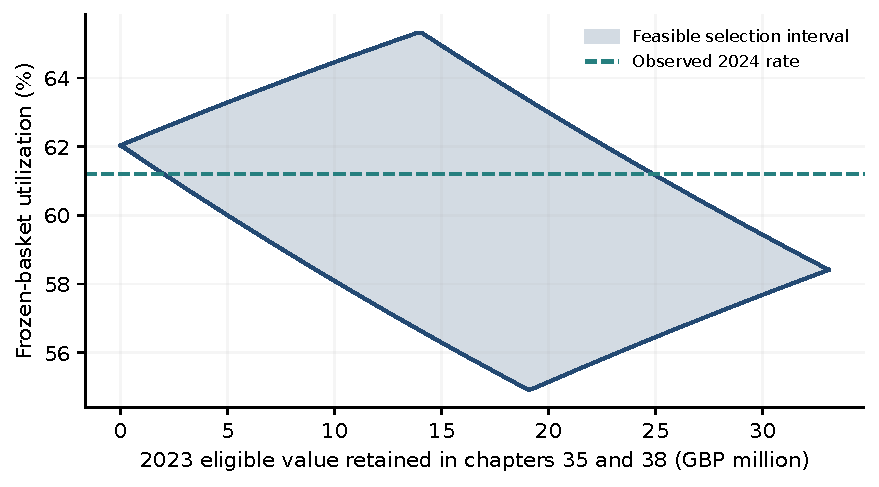
\includegraphics[width=.94\linewidth]{06_fixed_retention.pdf}
\caption{How additional information about mixed-chapter retention would tighten the 2023 benchmark. The shaded region is equation~\eqref{eq:fixed}. Its horizontal coordinate concerns retained value on the frozen 2023 basket, not observed 2024 trade value.}\label{fig:fixed}
\end{figure}

The minimum \MinSelection\-point increase across the unrestricted 2023 selection interval is robust to every used/unused allocation allowed by the coarse information set. It is not a claim that at least \MinSelection\ points of the realized increase were caused by reform. Realized trade, claims, and composition differ from the frozen basket. Keeping this distinction explicit prevents a mechanical benchmark from being converted into a causal attribution.

\section{Broader comparisons and sensitivity}
\subsection{Opposing aggregate and chapter-rate changes}
In the broader matched sample, 33 of \PanelCount\ panels have opposite signs for the total change and the rate component. Sixteen meet the additional 0.5-point materiality threshold for both changes. Figure~\ref{fig:panels} displays every selected panel, including non-reversals. Table~\ref{tab:examples} lists the six material reversals with the largest absolute total changes.

\begin{figure}[!htbp]
\centering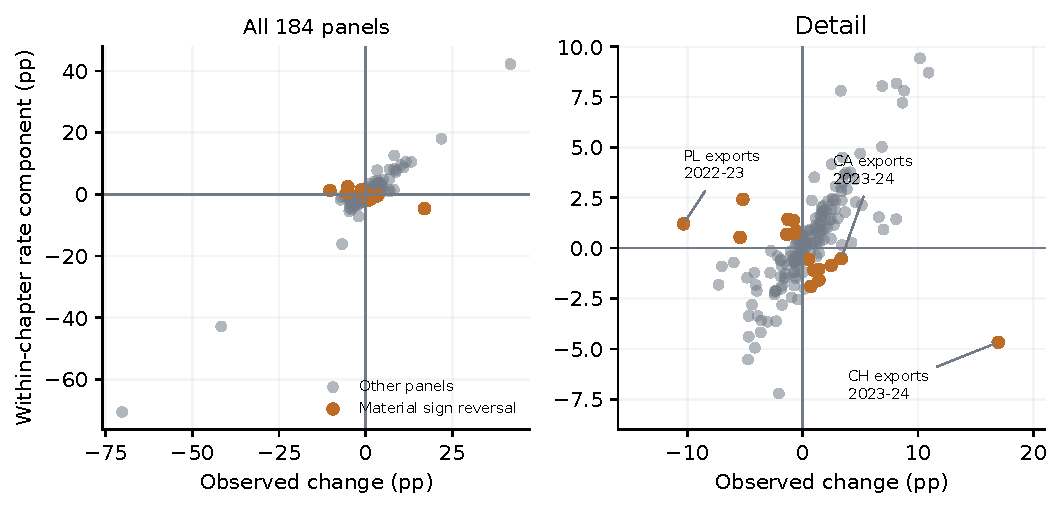
\includegraphics[width=\linewidth]{05_panel_reversals.pdf}
\caption{Aggregate versus within-chapter utilization changes in \PanelCount\ material matched panels. The right panel enlarges the central region; all observations appear in the left panel. Orange points have opposing signs with both changes at least 0.5 percentage point in magnitude. Panels use 2022--23 and 2023--24. Repeated partners and directions are not independent replications.}\label{fig:panels}
\end{figure}
\begin{table}[!htbp]
\centering
\caption{Largest material sign reversals in the eligible panel}\label{tab:examples}
\small
\begin{tabular}{lllrrrr}
\toprule
Partner & Direction & Period & Total & Rates & Weights & Exit \\
\midrule
CH & exports & 2023--24 & +16.94 & -4.68 & +7.46 & +14.16 \\
PL & exports & 2022--23 & -10.31 & +1.20 & -11.54 & +0.00 \\
MK & exports & 2022--23 & -5.42 & +0.54 & -5.96 & +0.00 \\
MT & exports & 2022--23 & -5.17 & +2.42 & -7.59 & +0.00 \\
CA & exports & 2023--24 & +3.34 & -0.52 & +3.87 & -0.00 \\
CR & imports & 2022--23 & +1.42 & -1.58 & +3.00 & +0.00 \\
\bottomrule
\end{tabular}
\par\vspace{3pt}\begin{minipage}{.97\linewidth}\footnotesize Percentage points. CH: Switzerland; PL: Poland; MK: North Macedonia; MT: Malta; CA: Canada; CR: Costa Rica. These six panels have the largest absolute total changes among material reversals. All displayed entry contributions round to zero except Poland (2022--23), at +0.03 pp. Direction refers to UK trade. The full file includes all eligible panels, including non-reversals.\end{minipage}
\end{table}


For UK exports to Poland in 2022--23, utilization declines by 10.31 points while the within-chapter rate component rises by 1.20 points. Changing weights contribute $-11.54$ points. For exports to Canada in 2023--24, the aggregate rises by 3.34 points while the rate component declines by 0.52 point, offset by a 3.87-point weight contribution. These examples establish accounting reversals without establishing a common underlying policy mechanism. The Swiss case is distinctive because the legal tariff change independently explains a broad loss of industrial eligibility.

\subsection{Value thresholds, weighting, and aggregation}
Table~\ref{tab:sensitivity} varies the eligible-value cutoff while keeping the 0.5-point change criterion. Material reversal shares range from 5.4\% to 8.7\%. The package also supplies 0.1- and 1-point change thresholds. These counts depend on the comparison universe. They should not be interpreted as the prevalence of misleading policy evaluation in all UK agreements.
\begin{table}[!htbp]
\centering
\caption{Sensitivity of the descriptive reversal count}\label{tab:sensitivity}
\small
\begin{tabular}{rrrr}
\toprule
Eligibility cutoff & Panels & Reversals & Share (\%) \\
\midrule
\pounds25m & 232 & 20 & 8.6 \\
\pounds50m & 212 & 17 & 8.0 \\
\pounds100m & 184 & 16 & 8.7 \\
\pounds250m & 144 & 9 & 6.2 \\
\pounds500m & 112 & 6 & 5.4 \\
\bottomrule
\end{tabular}
\par\vspace{3pt}\begin{minipage}{.97\linewidth}\footnotesize Both years must meet the eligibility cutoff. All panels are partner--direction--year-pair observations for 2022--23 or 2023--24, have at least 99\% matched eligibility coverage in each year, and have a common eligible support. A material reversal requires opposite signs and magnitudes of at least 0.5 pp for both the aggregate change and the within-chapter rate component. Repeated partners are not independent observations.\end{minipage}
\end{table}


For Swiss agriculture, weighting continuing chapters by either their 2023 or 2024 eligible values gives rate changes of $-0.875$ and $-0.853$ point. Equal chapter weights instead give $+2.546$ points. An average chapter and an average pound of eligible trade answer different questions. The main estimand is trade-value weighted because the official utilization statistic is value weighted; the equal-weight result rules out a claim that utilization fell across chapters in a uniform sense.

Dropping each of the 20 agricultural chapters with positive baseline eligibility in turn leaves the symmetric agricultural rate component negative in every case. The raw agricultural aggregate change remains negative in 19 of the 20 restrictions and becomes slightly positive when chapter 18 is omitted. These checks distinguish the stability of the weighted rate component from the greater sensitivity of an unstandardized aggregate.

Coarsening HS2 chapters to HS sections also reallocates the accounting components. For Switzerland in 2023--24, the rate component remains negative, at $-13.71$ points, while weights contribute $+26.96$ and section-level exit $+3.69$ points. The total remains $+16.94$. For Poland in 2022--23, the positive chapter-rate component becomes a negative section-rate component. Canadian exports in 2023--24 also change the sign of the rate component on aggregation. Thus the general-panel reversal count is a result at a declared product resolution, not an invariant measure of behavioral change. The legal frozen-basket Swiss bound provides information that purely statistical coarsening does not.

\section{Economic and commercial interpretation}
\subsection{A utilization target need not rank lower private costs}
The accounting concern matters for how policy targets and commercial claims are framed. Consider a fixed unit of trade that can pay an MFN tariff $\tau\geq0$ or incur an origin-compliance cost $c\geq0$ to obtain a zero preferential tariff. A cost-minimizing importer incurs $\min\{c,\tau\}$. If a fraction $u$ claims preferences, removing the MFN tariff saves private tariff and compliance expenditure equal to
\begin{equation}
 B=x\big[(1-u)\tau+u\bar c\big],
 \label{eq:private}
\end{equation}
where $x$ is trade value and $\bar c$ the mean per-value compliance cost among claimants. This stylized expression assumes compliance expenditure is avoidable after removal and abstracts from quantities, prices, and continuing documentation obligations. Tariff payments are transfers from a national-welfare perspective, so $B$ is a private-cost measure, not a welfare statistic.

Equation~\eqref{eq:deletion} ranks removal by whether the removed pool's utilization is below the retained average. Equation~\eqref{eq:private} depends additionally on tariffs and compliance costs. The rankings can conflict even when every observed claiming choice is privately optimal. For two equal-value pools with utilization 0.2 and 0.8, the starting aggregate is 0.5. Removing the low-use pool raises utilization to 0.8; removing the high-use pool lowers it to 0.2. If the low-use pool has $\tau=0.01$, $\bar c=0.005$, its private saving per unit value is 0.009. If the high-use pool has $\tau=0.20$, $\bar c=0.10$, its saving is 0.12. Assign non-claimants costs above their tariff in each pool to make both choices rational. The reform with the greater private saving lowers measured utilization. The numbers are an analytical example, not a calibration to Swiss firms.

\subsection{Implications for agreement monitoring and compliance software}
A useful policy report can retain the familiar utilization statistic while supplying the information needed to interpret it: eligible and used values; the support entry/exit ledger; standardized rates at a stated product resolution; and tariff-free access split between MFN and preferences. The Swiss case shows why all of these are useful. A high final utilization rate can coincide with a much smaller remaining population in need of agreement-specific treatment.

For trade-compliance providers, the equivalent distinction is between preference adoption and a change in the need for a preference. Crediting an automated qualification product with every observed utilization increase would be inappropriate when MFN liberalization changes the denominator. Conversely, a platform that correctly stops soliciting origin evidence after tariff abolition may deliver savings while recording fewer preferential transactions. Evaluation should separate tariff changes, new qualifying evidence, processing-regime changes, and changes in client product mix.

This application operates in an existing market. Public agreement-use dashboards and commercial FTA qualification tools already exist \citep{secomonitor2026,thomson2026,descartes2026}. The replication code supplies an auditable aggregate reporting component. It does not demonstrate customer willingness to pay, product-market fit, a legal origin determination, patentability, or a validated estimate of recoverable duties. Shipment-level rates, origin evidence, and processing arrangements would be required for those further claims.

\section{Limitations and research implications}
The central empirical result is conditional on the official aggregates and their reported classifications. We have verified source integrity, arithmetic, coverage, and several published controls, but cannot independently audit the customs declarations underlying the statistics. The source-year quarantine illustrates why provenance must remain visible even for official workbooks.

The design identifies an accounting reversal and a fixed-basket compatibility interval. It does not identify the counterfactual path of Swiss preference use without reform. No difference-in-differences interpretation is attached to a country whose product eligibility changed sharply; there is no firm-level panel, randomly assigned compliance intervention, or estimated private cost distribution. The observed agricultural decline should not be projected onto the industrial firms that left the measured population.

HS2 aggregation is both a practical advantage and a limit. It permits exact public replication, but mixed product chapters require bounds and positive-eligibility chapters can conceal changes in underlying tariff lines. Tariff-line concordances and dated legal measures would improve the selection benchmark. Linked firm--product declarations would then permit a distinct behavioral study of claim choices on stable eligibility. That would be a different estimand from the exercise reported here.

The general-panel findings also depend on materiality thresholds, matching, and product resolution. We disclose results that weaken an overly broad interpretation: equal chapter weighting reverses the sign of the Swiss agricultural rate change, and section aggregation reverses some country-level classifications. The robust claim is narrower: trade-value utilization progress cannot be read off the headline conditional ratio when eligibility and composition change, and the Swiss reform supplies a quantitatively important, reproducible instance.

\section{Conclusion}
Switzerland's industrial tariff abolition reduced the need for preferential tariff treatment on most UK industrial exports. Reported utilization increased by 16.94 percentage points while eligible trade fell by 92.52\%. Agricultural utilization declined, and the full chapter decomposition has a negative rate component. Even after allowing unresolved agricultural content in the two mixed chapters, selection alone on the fixed 2023 basket can generate a rate spanning the observed 2024 outcome.

These findings support a specific change in evaluation practice: report the eligible population and its support changes alongside preference utilization, and distinguish tariff-free access from agreement-specific claiming. The distinction preserves the economic meaning of tariff liberalization and prevents a changing denominator from becoming evidence for a behavioral mechanism that the aggregate data cannot establish.

\paragraph{Data and code availability.}
The public replication repository contains the archived official workbooks with attribution, the source manifest, parsed and quarantined data, analysis and figure scripts, numerical outputs, and verification tests. All reported numerical exercises can be run without private data, model-service credentials, or paid data access. No external funding was received for this computational work.

\FloatBarrier
\begin{thebibliography}{99}
\bibitem[Ayele et al.(2023)]{ayele2023} Ayele, Y., Gasiorek, M., and Tong Koecklin, M. (2023). Trade preference utilization post-Brexit: The role of rules of origin. \emph{World Trade Review}, 22(3--4), 436--451. \href{https://doi.org/10.1017/S1474745623000228}{doi:10.1017/S1474745623000228}.
\bibitem[Brenis et al.(2024)]{brenis2024} Brenis, A., Gasiorek, M., and Tong Koecklin, M. (2024). \emph{How Much Free Trade in UK Free Trade Agreements?} UK Trade Policy Observatory Briefing Paper 83. \href{https://blogs.sussex.ac.uk/uktpo/publications/how-much-free-trade-in-uk-free-trade-agreements/}{Online source}.
\bibitem[Cariola and Lanz(2022)]{cariola2022} Cariola, G., and Lanz, R. (2022). \emph{Preference Utilization in the Global Economy: An Empirical Analysis}. WTO Staff Working Paper ERSD-2022-4. \href{https://www.wto.org/english/res_e/reser_e/ersd202204_e.pdf}{Online source}.
\bibitem[Charnes and Cooper(1962)]{charnes1962} Charnes, A., and Cooper, W. W. (1962). Programming with linear fractional functionals. \emph{Naval Research Logistics Quarterly}, 9(3--4), 181--186. \href{https://doi.org/10.1002/nav.3800090303}{doi:10.1002/nav.3800090303}.
\bibitem[Conconi et al.(2018)]{conconi2018} Conconi, P., Garc\'ia-Santana, M., Puccio, L., and Venturini, R. (2018). From final goods to inputs: The protectionist effect of rules of origin. \emph{American Economic Review}, 108(8), 2335--2365. \href{https://doi.org/10.1257/aer.20161151}{doi:10.1257/aer.20161151}.
\bibitem[Department for Business and Trade(2026a)]{dbt2026a} Department for Business and Trade (2026a). \emph{Preference Utilisation of UK Trade in Goods}. Official statistical collection, databases for 2021--2024, retrieved 16 October 2026. \href{https://www.gov.uk/government/collections/preference-utilisation-of-uk-trade-in-goods}{Online source}.
\bibitem[Department for Business and Trade(2026b)]{dbt2026b} Department for Business and Trade (2026b). \emph{Preference Utilisation of UK Goods in 2024}. Published 23 April 2026. \href{https://www.gov.uk/government/statistics/preference-utilisation-of-uk-trade-in-goods-2024/preference-utilisation-of-uk-goods-in-2024}{Online source}.
\bibitem[Department for Business and Trade(2026c)]{dbtannex2026} Department for Business and Trade (2026c). \emph{Preference Utilisation of UK Trade in Goods: Official Statistics Technical Annex}. Updated 23 April 2026. \href{https://www.gov.uk/government/statistics/preference-utilisation-of-uk-trade-in-goods-technical-annex/preference-utilisation-of-uk-trade-in-goods-official-statistics-technical-annex}{Online source}.
\bibitem[Descartes(2026)]{descartes2026} Descartes (2026). \emph{Descartes Introduces New AI-Powered Free Trade Intelligence (FTI) Solution to Help Reduce Trade Costs}. Product announcement, accessed 16 October 2026. \href{https://www.descartes.com/resources/news/descartes-introduces-new-ai-powered-free-trade-intelligence-fti-solution-help-reduce?language=en}{Online source}.
\bibitem[Gonciarz and Verbeet(2025)]{gonciarz2025} Gonciarz, T., and Verbeet, T. (2025). \emph{Significance of Most-Favoured-Nation Terms in Global Trade: A Comprehensive Analysis}. WTO Staff Working Paper ERSD-2025-02. \href{https://www.wto.org/english/res_e/reser_e/ersd202502_e.pdf}{Online source}.
\bibitem[Keck and Lendle(2012)]{keck2012} Keck, A., and Lendle, A. (2012). \emph{New Evidence on Preference Utilization}. WTO Staff Working Paper ERSD-2012-12. \href{https://www.wto.org/english/res_e/reser_e/ersd201212_e.pdf}{Online source}.
\bibitem[Kitagawa(1955)]{kitagawa1955} Kitagawa, E. M. (1955). Components of a difference between two rates. \emph{Journal of the American Statistical Association}, 50(272), 1168--1194. \href{https://doi.org/10.1080/01621459.1955.10501299}{doi:10.1080/01621459.1955.10501299}.
\bibitem[Krishna et al.(2025)]{krishna2025} Krishna, K., Salamanca, C., Suzuki, Y., and Volpe Martincus, C. (2025). Learning to use trade agreements. \emph{Journal of Development Economics}, 174, 103424. \href{https://doi.org/10.1016/j.jdeveco.2024.103424}{doi:10.1016/j.jdeveco.2024.103424}.
\bibitem[Legge and Lukaszuk(2024)]{legge2024} Legge, S., and Lukaszuk, P. (2024). The firm-level costs of utilizing free trade agreements. \emph{International Economics}, 178, 100484. \href{https://doi.org/10.1016/j.inteco.2024.100484}{doi:10.1016/j.inteco.2024.100484}.
\bibitem[Office for National Statistics(2025)]{ons2025} Office for National Statistics (2025). \emph{Use of Preferential Tariffs by UK Businesses for Imports of Goods: 2012 to 2023}. Released 9 October 2025. \href{https://www.ons.gov.uk/businessindustryandtrade/internationaltrade/articles/useofpreferentialtariffsbyukbusinessesforimportsofgoods/2012to2023}{Online source}.
\bibitem[SECO(2026a)]{seco2026} State Secretariat for Economic Affairs (2026a). \emph{Abolition of Industrial Tariffs}. Official policy description and questions and answers, accessed 16 October 2026. \href{https://www.seco.admin.ch/en/industrial-tariffs-abolition}{Online source}.
\bibitem[SECO(2026b)]{secomonitor2026} State Secretariat for Economic Affairs (2026b). \emph{Use of Free Trade Agreements}. Official methodology and monitoring overview, accessed 16 October 2026. \href{https://www.seco.admin.ch/en/use-of-free-trade-agreements}{Online source}.
\bibitem[Tamberi and Tong Koecklin(2022)]{tamberi2022} Tamberi, N., and Tong Koecklin, M. (2022). \emph{Preference Utilisation in the TCA: How Are We Doing?} UK Trade Policy Observatory Briefing Paper 72. \href{https://blogs.sussex.ac.uk/uktpo/files/2022/12/BP-72-v2.pdf}{Online source}.
\bibitem[Thomson Reuters(2026)]{thomson2026} Thomson Reuters (2026). \emph{Free Trade Agreement Management}. ONESOURCE product description, accessed 16 October 2026. \href{https://africa.thomsonreuters.com/en/products-services/global-trade-management/free-trade-agreement.html}{Online source}.
\end{thebibliography}

\appendix
\section{Verification and replication details}
\subsection{Independent checks of the selection bounds}
The verification suite enumerates 1,980 small integer configurations. Retained eligibility ranges from 1 to 8, its used value ranges from zero to that eligibility, ambiguous eligibility ranges from zero to 8, and ambiguous used value covers every feasible integer. For every configuration we enumerate every integer retained-used and retained-unused pair and compare the exact rational extrema to equation~\eqref{eq:bounds}. We also check every integer total-retention constraint against equation~\eqref{eq:fixed}. These are mathematical verification cases, not observations about trade.

A separate numerical check applies the linear-fractional transformation of \citet{charnes1962}. Let $t=(e+v+w)^{-1}$, $z=vt$, and $h=wt$. Then the lower endpoint solves
\begin{align}
 \min_{z,h,t\geq0}\quad &pt+z\\
 \text{subject to}\quad &et+z+h=1,\\
 &z\leq qt,\qquad h\leq(a-q)t.
\end{align}
Maximizing the same objective gives the upper endpoint. Two hundred seeded continuous configurations are solved with the HiGHS linear-programming implementation and compared to the closed forms to nine decimal places. We use the optimizer as an independent implementation check, not as a source of additional empirical precision.

For the decomposition, 1,000 seeded nonnegative integer panels are evaluated with independent rational arithmetic and compared to the numerical implementation. The rational identity closes exactly. The largest floating-point accounting residual over the retained empirical comparisons is less than $2\times10^{-16}$ in rate units. Cases with no common eligible support, missing values, invalid use exceeding eligibility, or a zero retained denominator are rejected explicitly.

\subsection{Source and pipeline checks}
Each raw archive file is checked against its saved SHA-256 digest, and parsed row counts are compared to the manifest. Canonical values are read from the ODS numeric attributes, preserving the distinction between numeric zero and missing data. The ISO code NA is retained as Namibia, not interpreted as a missing-value marker. Original Year fields are checked against release-file years before analysis. Source mismatches are archived separately and never silently recast as valid observations.

Independent controls use rounded values from DBT's 2024 published commentary: Swiss and Japanese eligible/use exports, and Swiss and Japanese eligible/use imports, together with their reported utilization rates. The package's aggregates agree within the publication's rounding intervals. There are seven automated test methods in total; the exhaustive and optimization checks run within those methods. A saved verification log accompanies the results.

\subsection{Reproduction commands}
From the repository root, install the pinned Python dependencies in an isolated environment, then run:
\begin{verbatim}
python src/analyze.py
python src/figures.py
python src/report.py
python -m unittest discover -s tests -v
cd paper
tectonic manuscript.tex
\end{verbatim}
The archived inputs make the main replication independent of later revisions to the government website. The optional acquisition script can retrieve the current releases and rebuild parsed tables; a new release should be stored as a new data vintage rather than overwriting this study's archive. The source manifest and README give exact dependency versions, input locations, and output definitions. Figures are vector PDFs and are generated from saved numerical outputs.

\section{An allocation witness for the 2023 compatibility result}
Let $u^*=P_{2024}/E_{2024}$ be the observed 2024 rate. In the 2023 frozen-basket exercise, set retained-used ambiguous value $v=0$. Retaining unused ambiguous value
\begin{equation}
 w^*=\frac{p}{u^*}-e
\end{equation}
then reproduces the final ratio exactly. The archived values give $w^*\approx\pounds2.00$ million, which lies between zero and $a-q=\pounds19.09$ million. This supplies a feasible accounting witness for overlap with the observed rate. It does not establish that the witness corresponds to the Swiss agricultural tariff exceptions, or that the realized reform left behavior unchanged.

The distinction is empirically useful. A single illustrative removal rule can demonstrate possibility but may depend on an arbitrary classification of mixed chapters. The bounds quantify every allocation permitted by the coarse information, and the witness establishes attainable overlap rather than relying solely on visual proximity. Both statements remain conditional on a fixed historical basket.
\end{document}
